\chapter{Introduction}
\label{chap:scaling_introduction}

\begin{flushright}{\slshape    
The allometric law promises to become\\
an integral part of geography theory.} \\ \medskip
--- David Harvey (1969)~\cite{Harvey:1969} 
\end{flushright}


Another possibility is to look at the way
the system behaves when we change its size. That is, trying to see whether there
exists a function $f$ such that the quantity $Y$ varies as

\begin{equation}
    Y = f(S)
\end{equation}

where $S$ is the size of the system. If the function $f$ is relatively
simple---as power law are--- this hints at universal underlying behaviours that
are responsible for the behaviour of the system. Functional laws are are a trace
of the behaviour of the underlying system. The identification of functional laws
has several prerequisites however. The first one, is to be able to identify the
system. While this is trivial in the case of animals (it is fairly easy for us
to isolate an elephant, or a cat from its environment to measure its mass and
its metabolic rate), it is a much more difficult task in the case of cities.
Indeed, cities do not have fixed boundaries, the geographical limits of the
object studied evolves with time, as people are born and die, change residence
and as companies do the same. Traditionnally, people have relied on the
definition given by statistical agencies of the respective countries they were
studying---and we will do the same in the next chapter. We will however see, in
the chapter concluding this part, that the problem of delineating cities is a
sensible issue and affects greatly scaling analyses. A second issue, rarely---if
ever---mentionned in the literature, is the necessity to define the set of
cities to study. Scaling laws are essentially cross-sectional relationships,
studying the All studies take it as a given that we should look for scaling laws
does it make sense to mix French cities, Ukrainian, Canadian and Korean, etc
cities and plot, say, their total GDP as a function of the population? Would we
then observe a neat scaling relationship? Intuitively, one can see that this is
very unlikely to happen, as different countries have different levels of wealth,
and this should be reflected in the wealth of their cities. Therefore, plotting
cities from different countries together is likely to introduce important
deviations to the pure scaling relations which are not due to the fact that
cities in different countries do not follow the same processes, but rather
because of systemic differences at the country level. As a matter of fact, most
studies limit themselves to a single country. This question of the relation
between scaling relationships and countries will be dealt with partially in the
concluding chapter.  Finally, the last prerequisite is to know wht to use as
$S$, the size of the system. All studies plot quantities as a function of the
population size of cities, but we could also consider that the size of the city
is its spatial footprint, measured by its surface area $A$, or the total volume
of its buildings, etc. So why the population size? Behind this choice is implied
the realisation that cities are more than roads and buildings, cities are the
people who inhabit them. People are responsible for the changes in wealth,
employment, number of patents. People need new roads, and it is people who build
them. People need electricity, and again it is people who run electric cables
between buildings. Inhabitants in a city are the elements that interact
constantly, and in their actions and interactions are reponsible for the
collective mechanisms that act on a larger scale on the city as a whole. In a
sense, in the use of the population $P$ to measure the size of a city as a
system hides the understanding that cities are the people that inhabit them.

\begin{figure}
    \centering
    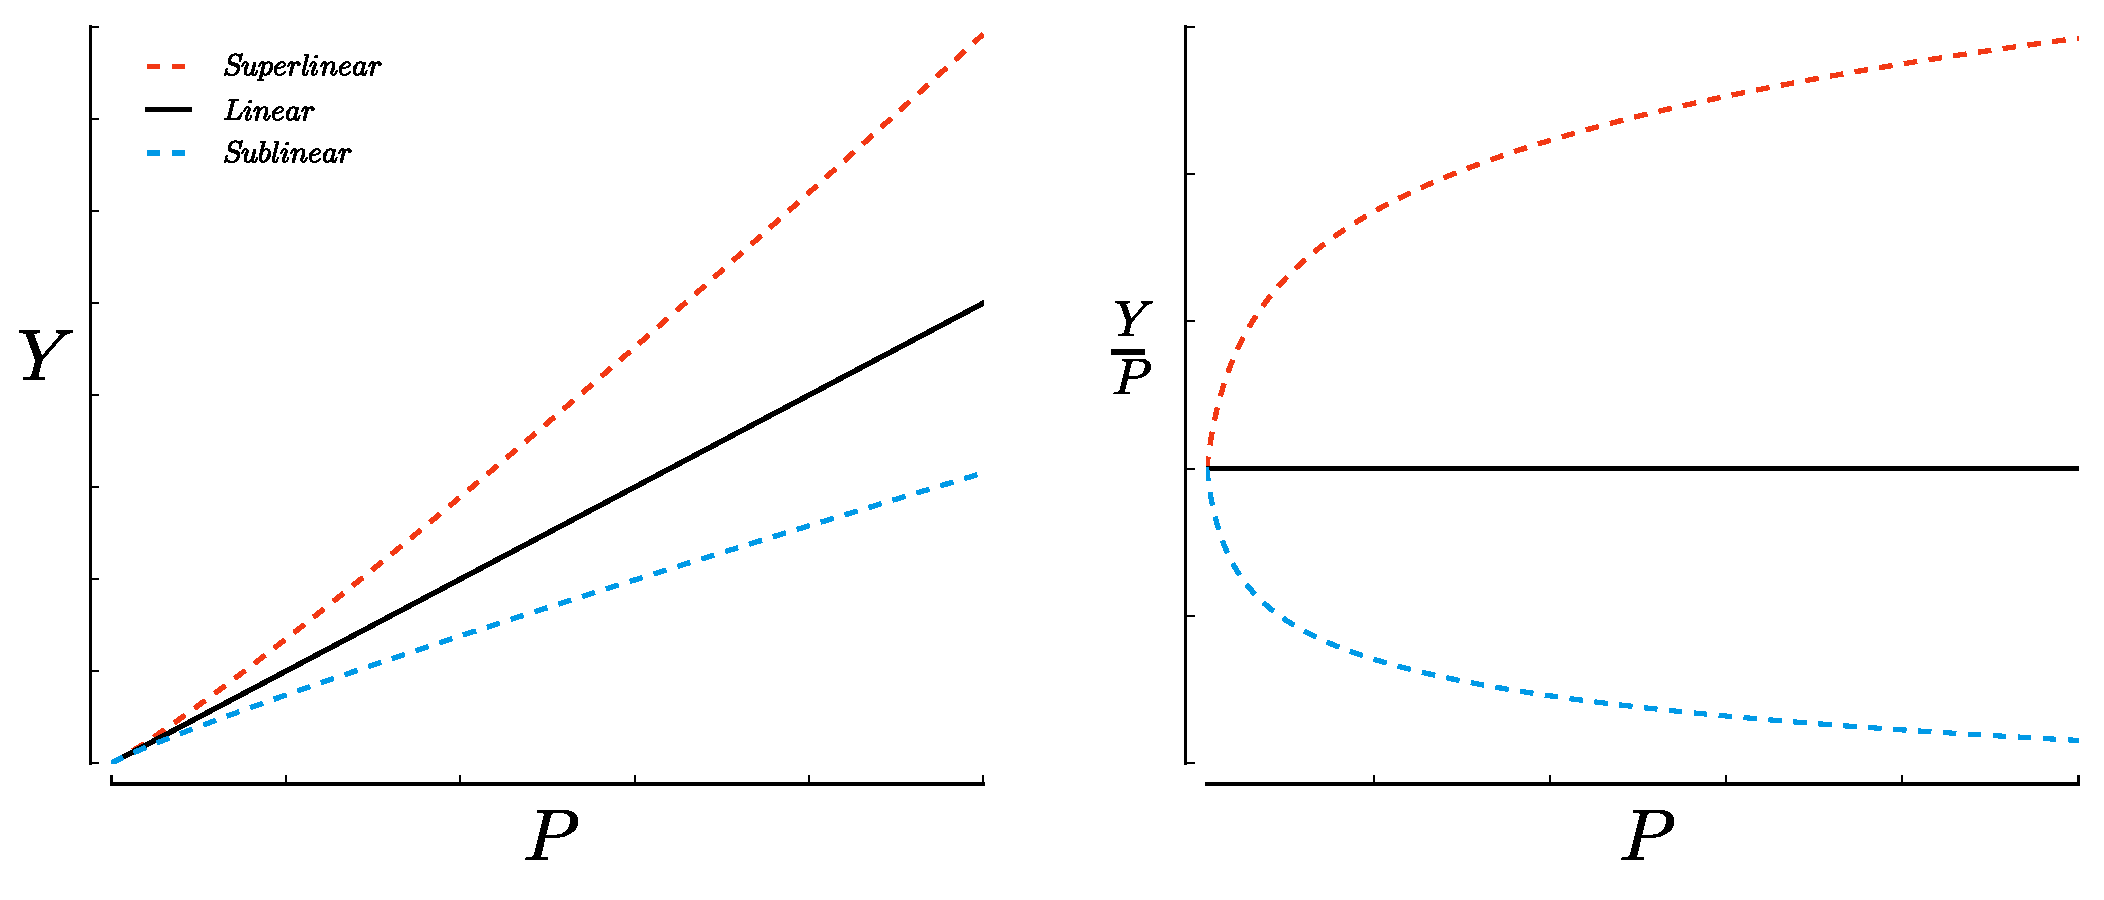
\includegraphics[width=\textwidth]{gfx/chapter-scaling/scaling_scheme.pdf}
    \caption{(Left) Example of a linear (black), sublinear (blue) and superlinear (red)
    behaviour. (Right) Evolution of the correspondant per-capita quantities with
population. A superlinear behaviour means that per-capita quantity increase with
population size, while a sublinear behaviour means per-capita quantities
decrease with city size.\label{fig:scaling_scheme}}
\end{figure}

Allometric scaling laws are, in a sense, the easiest way to probe a system in a
quantitative way. Assuming 

present themselves in the form of a power-law
relationship between various quantities $Y$ and the population size $P$ of
cities \emph{in a given system of cities} 

\begin{equation}
    Y = Y_0\,P^{\,\beta}
    \label{eq:scaling_definition}
\end{equation}

where the exponent $\beta$ can be different from $1$. This type of scaling
relation, used extensively in Biology~\cite{Thompson:1942} and in
Physics~\cite{Barenblatt:1996}, is a signature of the various processes
governing the phenomenon under study, especially when the exponent $\beta$ is
different from what would be naively expected. Three qualitatively different regimes are
usually
distinguished for the exponent $\beta$~\cite{Bettencourt:2007}

\begin{description}
    \item[Superlinear] when $\beta>1$. In this situation, the $Y$ per capita
        increases with population size. This is associated with the notion of
        increasing returns with scale in economics.
    \item[Linear] when $\beta=1$. In this situation, the $Y$ per capita is
        constant. This behaviour is characteristic of an extensive system, when
        the whole is nothing but the sum of its parts.
    \item[Sublinear] when $\beta<1$. In this situation, the $Y$ per capita
        decreases with population size. When $Y$ is the cost in infrastructure,
        this is characteristic of economies of scale.
\end{description}    

The scaling exponent $\beta$ is also directely related to the \emph{elasticity}
defined in Economics. Indeed, we have

\begin{equation}
    \beta = \frac{dY/Y}{dP/P}
\end{equation}

Which is the definition of cities' population elasticity of $Y$. Their application to the study of cities
is not recent~\cite{Stewart:1947}, but has undoubtedly caused a stir in the
literature about urban systems over the last decade.\\

The epigraph used at the beginning of this chapter, found in Harvey's 1969
\emph{Explanation in Geography}, is somewhat prophetic.  Allometric scaling
relationships only concern $1$ page out of the $500$ pages that the book
contains, a reflection of the very few empirical results that were available at
the time.  Looking at the extent of the literature on scaling relationships
almost $50$ years after Harvey wrote this sentence, it is difficult to deny the
veracity of this prophecy. Thanks to the wider availability of data through
statistical agencies, but also the availability of 'new data' (such as mobile
phone data), empirical measurements of scaling laws have multiplied,
and now concern quantities as diverse as the total surface area, the number of
patents, the quantity of $CO_2$, the number of phone contacts of individuals, etc. Yet, despite the current empirical wealth, different theoretical interpretations of these scaling laws are currently in competition, between the transversal interpretation put forth by geographers~\cite{Pumain:2006} and the longitudinal interpretations more recently defended by physicists~\cite{Bettencourt:2013, Louf:2014_smog}.  In this introductory chapter, I will begin with a brief, non exhaustive historical review of the empirical results on scaling relationships. I will then discuss the existing theoretical frameworks. I will argue that the various interpretations given to scaling laws are not necessarily incompatible with one another, but rather they provide different explanations to different phenomena.  This will lay the ground for our contribution to the debate, and a theoretical interpretation of the scalings related to the mobility of people, and an estimate for the scaling exponent of the surface area.  \section{A brief history of allometric scaling and cities} \label{sec:a_brief_history_of_allometric_scaling_and_cities} In this section, I will proceed to give an historical overview of scaling relationships in the literature. Rather than an exposition that is linear in time, I deliberately chose to classify the proposed relationship in various categories in order to emphasize the variety of variables that have been studied, as well as the curious waves of interest and disinterest in the history.  
\subsection{Surface area}
\label{sub:surface_area}

One of the first quantities one can think of is the spatial footprint of cities,
as can be observed on satellite pictures, or maps. It is therefore not
surprising that the first occurence of the scaling relationship in the study of
cities concerns the study of the scaling of the surface area of cities with
their population, drawn in $1947$ from data for administrative cities obtained
from the 1940 US Census.  Funnily enough, the author of the
study~\cite{Stewart:1947}, John Stewart, was a physicist.

\begin{equation}
    A = \frac{P^{\,3/4}}{350}
\end{equation}

The next occurence of this relationship can be found $9$ years later in a study
led by the same author~\cite{Stewart:1958}, using UK census data, and published
in a more specialised journal. From there, it isn't long until the result
percolates in geographywith Boyce in~\cite{Boyce:1963}.  Nordbeck's
paper~\cite{Nordbeck:1965} also studies the scaling of surface area with
population, and, for the first time, explicitly refers to allometry in biology.
Later, Tobler~\cite{Tobler:1969} uses some of the first available sateljite
images to provide the first confirmation using satellite pictures. Satellite
pictures were used more recently by Guerois in ~\cite{Guerois:2003}. When
applied to morphological definitions of cities within the same system of cities,
all the studies (see~\cite{Batty:2011}) give an exponent that varies in the
range $[0.70, 0.90]$, with a good statistical agreement. It seems however,
different results are obtained, and that such a simple statistical relationship
does not hold for functional definitions of cities~\cite{Batty:2011}, or when
cities span several systems of cities~\cite{Fuller:2009}.

Thus, despite being the oldest and most trusted scaling realtionship in the
literature, the relation between the surface area and population size of cities
exhibits some of the issues with scalings that we will talk about later.

\subsection{Economic diversity}
\label{sub:economic_diversity}

The economic diversity has been of interest to researchers very early on. In
1949, Zipf in \emph{Human behavior and the principle of least
effort}~\cite{Zipf:1949} plots the number of service-business, manufactures and
retail stores per city as a function of population (in log-log scale) using data
from the $1940$ US Census. He finds a linear relationship with population for
the three types of establishments, which agreed at the time with his model. He
also plots the diversity, defined as the number of different kinds of
entreprises present in the city being studied. In his 1967 \emph{Geography of
market centers and retail distribution}~\cite{Berry:1967} Berry, hoping to
demonstrate the hierarchical organisation of central places, plots this time
the population of cities as a function of the number of kinds of retail and
service businesses observed. Strangely enough, the data seem to show

\begin{equation}
    D \propto P^{\, \beta}
\end{equation}

with $\beta > 1$, in contradiction with later results found by Bettencourt et
al.~\cite{Bettencourt:2014}.\\

More recently, Pumain and coauthors~\cite{Pumain:2006}, extending the work done
by Fabien Paulus in his PhD thesis~\cite{Paulus:2004}, showed that the
employment in different activities in cities scaled as

\begin{equation}
    E_a \propto P^{\,\beta}
\end{equation}

with different exponents $\beta$ for the different activities. They observed,
for the year $1999$ in France, that the exponents could be classified in three
categories

\begin{itemize}
    \item $\beta > 1$ for innovative sectors: research and developpement,
        consultancy.
    \item $\beta = 1$ for common sectors: hotels, health and social services,
        education.
    \item $\beta < 1$ for `mature' sectors such as the food industry
\end{itemize}

This result was confirmed recently by Youn et al.~\cite{Youn:2014} (although
they do not refer to this previous work), who showed that the same behaviour was
observed for the number of business of a given type. A particularly interesting
result shown by Pumain et al.~\cite{Pumain:2006} is the evolution of the
different exponents with time, where we can see a clear increase of the
exponents for research and developpement, and a clear decrease of the exponents
related to manufactures of different kinds. This behaviour in time is the
starting point of the authors' evolutionary theory to explain scaling laws, that
we will discuss later in this introduction.\\

Finally, Bettencourt et al.\cite{Bettencourt:2014} showed that the professional
diversity $D$, measured as the number of professions of different kind in the
city considered, could be fitted by the following function

\begin{equation}
    D(N_e) = d_0\, \frac{\left(\frac{N_e}{N_0}\right)^\gamma}{1+\left(\frac{N_e}{N_0}\right)^\gamma}
\end{equation}

where $d_0$ is the size of the classification used in the data, $N_0$ is the
typical saturation size, and $\gamma$ is an exponent expressing the extent to
which new activities `appear' as the total employment increases. However,
because the authors do not propose any model, and because other functions fit
the data as well as the proposed function (see introduction), the parameters
obtained have no clear meaning.

\subsection{Wealth}
\label{sub:wealth}

Although the notion of increasing returns with the size of the agglomeration is
often discussed in economics, it is difficult to find an emprical proof in the
literature. The superlinear scaling of the GDP of american cities as a function of
their population may be the most striking example of such increasing
returns~\cite{Bettencourt:2007}. In the same article, Bettencourt et al. showed
that the number of patents (used as a proxy for creativity) also scaled
superlinearly with population size in the US.

Because larger cities create proportionally more wealth than smaller cities, we
can wonder whether this supplement of wealth allows to sustain proportionally
more jobs. The answer, as shown in~\cite{Bettencourt:2014} for american cities,
is negative: the total employment of a city is on average proportional to its population.

\subsection{Human interactions}
\label{sub:human_interactions}

At the heart of Bettencourt's model~\cite{Bettencourt:2013} to explain the
superlinear scaling of quantities associated with wealth and creativity is the
behaviour of the total number of interactions between individuals with the size
of the city. In an attempt to test this hypothesis, Schl\"apfer et
al.~\cite{Schlapfer:2014} looked at the scaling of the cumulative number of
contacts $K$ that people had over the phone, using mobile phone data in
Portugal, and landlines in the UK. They also looked at the cumulative call
volume (total number of minutes called) and the cumulative number of calls, and
found that the three quantities scale superlinearly with population size. They
further found that the number of non-returned calls showed a larger exponents
than the number of calls, meaning that the number of solicitations an individual
gets is greater in large cities.
Although this is not emphasized by the authors of the study, we note that the
exponents found in Portugal vary with the city definition that is chosen, with a
clear superlinear behaviour for Portugal's municipalities and `statistical
cities', but a near-linear behaviour for LUZ (Larger Urban Zones, a functionnal
definition of cities introduced by Eurostat).


\subsection{Mobility of individuals}
\label{sub:mobility}

The mobility of individuals in city has recently been the center of attention,
thanks to the recent availability of mobile phone data. Yet, most scaling
relationships that can be found in the literature were derived from traditional
census data, maybe because mobile phone data are granular, and authors naturally
tend to look at more specific quantities.
Also, because cars are universally used, and because peak travel demands on the
roads usually corresponds to journey-to-work trips, most of the information
available through surveys concern the commuting to work, often by car.
Hopefully, new data such as mobile phone data should be able to inform us about
other trips, which represent no less than 80\% of all trips undertaken in the
United States!~\cite{FHWA-PL-11-022}.

Samaniego and Moses~\cite{Samaniego:2008} showed that the total number of miles
driven in Urban Areas (morphological definition) in the US scaled sublinearly
with population size, with a non-trivial exponent (that is, different from
$1/2$. More details in the next chapter).  Also related to commuting and the use of
personal vehicles in general is the evolution of the total comsumption of
gasoline as a function of city sizes. Bettencourt et al. showed that gasoline
sales in Metropolitan Statistical Areas scaled sublinearly with population
size~\cite{Bettencourt:2007}. 

Finally, a diseconomy associated with the mobility of individuals is the
quantity of $CO_2$ emitted due to transportation (and polluting substances).
Using different city definitions, different authors find very different
behaviours. The authors of \cite{Fragkias:2013} find that transport-related
$CO_2$ emissions in Metropolitan Statistical Areas in the US scale sublinearly
with population size, while the authors of
~\cite{Louf:2014_mobility,Oliveira:2014} find that they scale superlinearly with
population size for US Urban Areas (morphological definition). Even more
confusing, the authors of~\cite{Rybksi:2013}, gathering data for many different
cities across the world, have found different scalings for developed and
developing countries. Although suggestive, we note that these results are based
on too few points to be conclusive. It is also not clear how to interpret
scaling relationships when cities from different systems of cities are
considered.


\subsection{Infrastructure}
\label{sub:infrastructure}

Studying the way the amount of infrastructure scales with population size is
interesting to know whether larger cities realise economies of scale, that is
whether cities are advantageous in the sense that we need to build less
roads, lay less cables for every individual.
The first study in this spirit was done by Veregin and Tobler, using the 1980 Us
Census DIME files (a lot less convenient to use than shapefiles) showed that the
number of street segments--the portion of road between two intersections--scaled
sublinearly with the size of urban areas~\cite{Veregin:1997}. Arguably, the
total length of the street network is more interesting to measure costs in terms
of infrastructure, and we have to wait until the study by Samaniego and Moses in
2008~\cite{Samaniego:2008}, to have evidence for the sublinear scaling of total
street length with the population size of urban areas. 

Finally, Bettencourt et al. showed that the length of electric cables in German cities
scaled sublinearly with population size~\cite{Bettencourt:2007}, indicating that
cities indeed realise some economies of scale.

\subsection{Basic commodities}
\label{sub:basic_commodities}

We can also wonder whether the consumption of basic commodities (housing, water,
electricity) per capita changes with population size. By far the most expected
result, Bettencourt et al. showed~\cite{Bettencourt:2007} that the total water
consumption (in China), the total electrical
consumption (in China),  and the total housing (in the US) are proportional to
the population.\\


A brief review of the literature is begging several questions. First, most of
the scaling exponents that are found in the literature (all but linear scalings)
are highly non-trivial, and it is not a-priori clear what mechanisms lead to
these values. Second, several studies find different exponent for the exact same
quantities, sometimes with a qualitative difference. For instance, the $CO_2$
emissions scale differently with population size in different studies. This
calls for an explanation.  As a more general remark, we can say that scaling
measures have been performed on a great variety of countries, at very different
times. Some exponents seem to keep the same value over time, while others are
obviously changing. We are therefore led to wonder the amount of confidence we
can have in these results.  As we will see, it depends on the situation. When
the empirical qualitative behaviour (i.e. superlinear, linear or sublinear) is
backed by an understanding of the underlying mechanisms (and a model), we have
more reason to trust it than a single empirical value. The issue of varying
qualitative behaviour for the same quantity we will see is the symptom of a
more fundamental problem in the study of urban systems (this is also the reason
why we cannot trust the exact value of scaling exponent, and cannot compare them
from one system of cities to another).



\section{Different phenomena, different explanations}
\label{sec:different_phenomena_different_explanations}
    
Recent wrks pretend explaining the origin of scalings in cities. However,
as should be clear from the literature reviews, scaling realtionships span
different phenomena that sometimes have very little to do with one another.
Rather than looking for a pseudo-universal interpretation of scaling laws, 

\cite{Pumain:2006} for an interpretation of scaling laws in terms of
innovation waves etc.

\cite{Bettencourt:2013} for the latest model to date.

The link between Eq.~\ref{eq:growth_resource_equation} is at best metaphorical.
But a metaphor is not a theory, and fancy language is not a substitute for a
real understanding of the system. As Einstein, Podolksy and Rosen succintly put
it in their famous critique of quantum mechanics~\cite{Einstein:1935}:

\begin{quote}
    In a complete theory there is an element corresponding to each element of
    reality.
\end{quote}

